\subsection{Core --- The Model for Sequences and Choices}\label{subsec:seqcore}
This section will present the model of Sequence focusing on the fields not presented in \myref{subsec:pictomodel}.

\myref{fig:sequencemodel} presents a class diagram of \texttt{Sequence} with the fields present.
We present the fields of the classes \texttt{Choice} and \texttt{Sequence} as these are the only classes which were not presented in \myref{subsec:pictomodel}.

\begin{figure}[!htb]
    \centering
    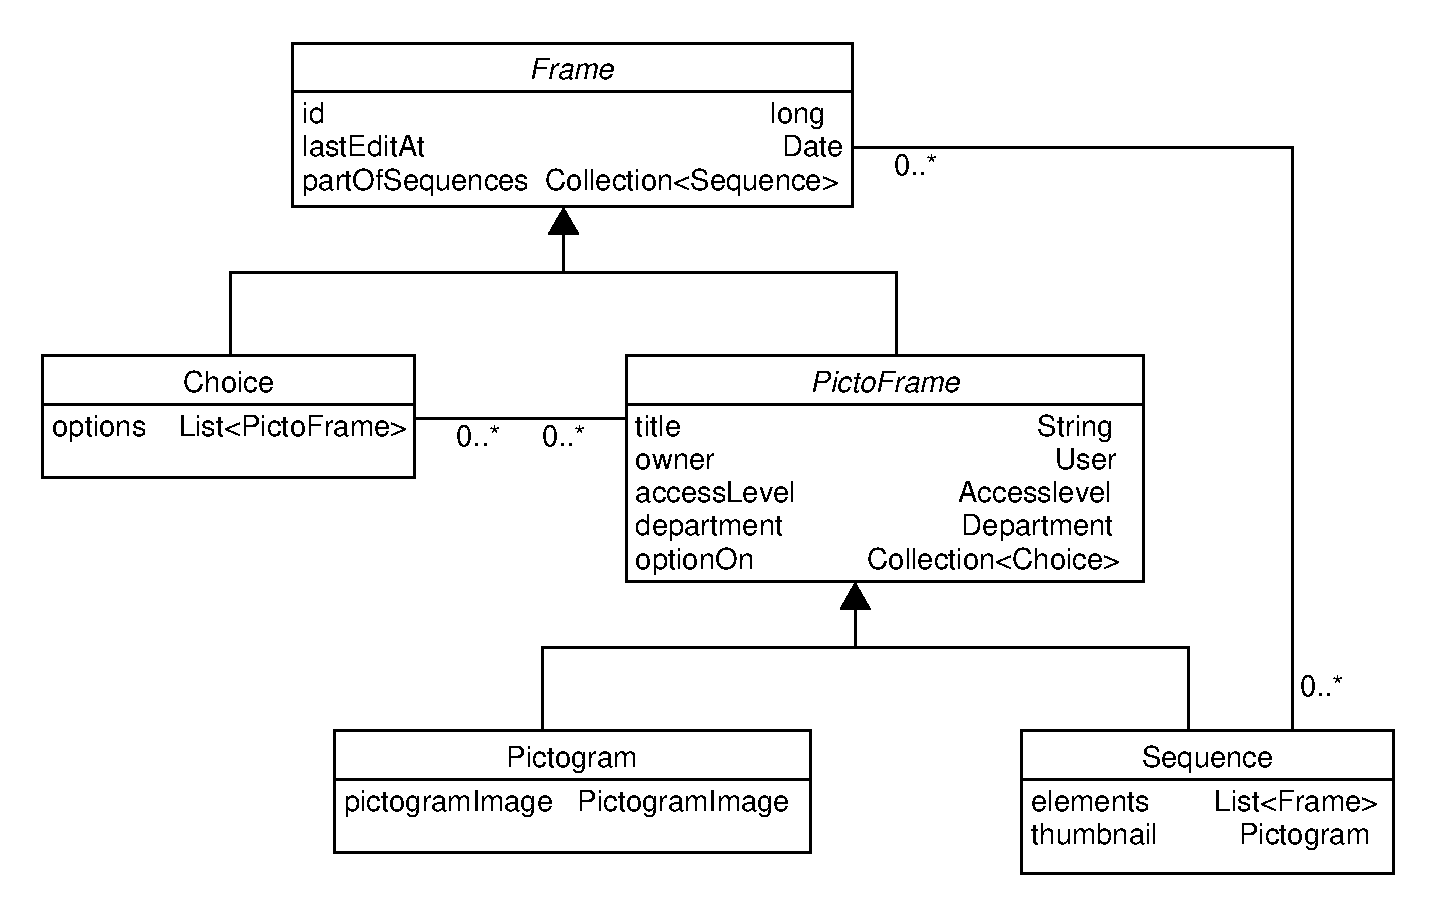
\includegraphics[width=0.8\textwidth]{figures/sequencemodel.pdf}
    \caption{Class--diagram including fields of the classes involved in Sequence}\label{fig:sequencemodel}
\end{figure}

\subsubsection{Sequence}
\begin{description}
	\item[elements] \hfill \\
    A list of \texttt{Frame}s stored on a \texttt{Sequence}.
	These are the \texttt{Frame}s that make up a sequence, it is therefore important that these are in a certain order.
	\item[thumbnail] \hfill \\
    This is the \texttt{Pictogram} which will be shown before beginning the \texttt{Sequence} in the app.
	This is simply a \texttt{Pictogram} with a \texttt{Many-To-One} relation.
\end{description}

\subsubsection{Choice}
\begin{description}
	\item[options] Like in a \texttt{Sequence} a \texttt{Choice} needs a list of elements, but unlike \texttt{Sequence} the list is made up of \texttt{PictoFrame}s which means a \texttt{Choice} cannot have nested \texttt{Choice}s.
    In order to retain the same behavior every time a \texttt{Choice} is used, the \texttt{options} list is ordered.
\end{description}
